%!TEX root = report.tex
The general structure of the code written for this exercise is shown in \cref{fig:3:structure}. Note that although the node \t{convert_rgb_to_gray_scale_server} is unconnected in this image, it has a link with \t{rgb_publisher}. Since it simply is a service and not an actual node publishing information, it shows as unconnected when a graph is generated. Below we discuss the route of an RGB image that is played from the bag file to the point where it is displayed in RGB and gray scale on the screen and the number of pixels in both those images have been counted. 



\begin{figure}
	\centering
	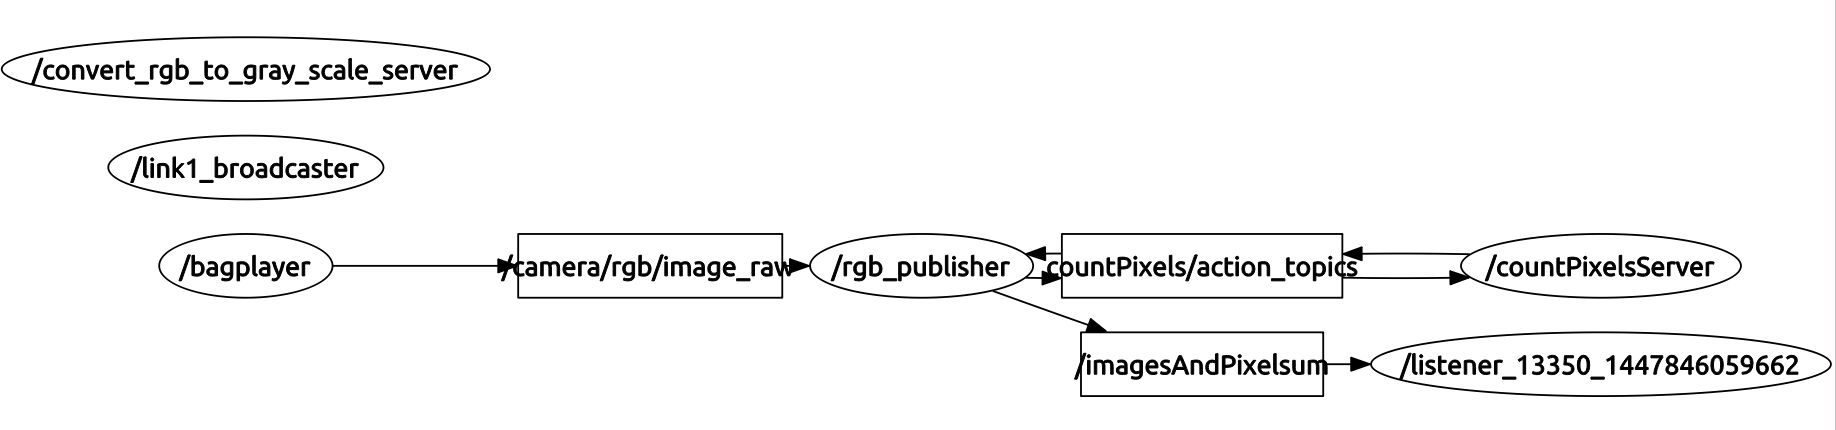
\includegraphics[width=\textwidth]{./img/3_structure}
	\caption{The connections between the different nodes.}
	\label{fig:3:structure}
\end{figure}

% rgb_publisher
In lieu of a camera the images are published from a bag, this is done by the node \t{bagplayer}. This nodes publishes RGB images on the topic \t{/camera/rgb/image_raw}. The \t{rgb_publisher} subscribes to this topic, see the method \t{subscriber_callback} in \cref{lst:3:publisher} in \cref{sec:a:ass3}. In the callback of this function, \t{subscriber_callback} the received RGB image is send to the \t{convert_rgb_to_gray_scale_server}. Since we only need to send the RGB image to this server we use the message type \t{sensor_msgs.msg.Image}. 

% rgb_to_gray_scale
The \t{convert_rgb_to_gray_scale_server} receives an RGB image and returns an grayscale image, both of type \t{sensor_msgs/Image}, see \cref{lst:3:RGBtoGrayScaleService}. The service converts the image to a CV image. The CV image is converted to a gray scale image which is converted back to the ROS image format, see \cref{lst:3:rgb_to_gray}. This image is send back to the requesting node as a \t{sensor_msgs.msg.Image}. We do not add the RGB image to the return message, since the requesting node already has this image. 

\lstinputlisting[
	caption={The \t{RGBtoGrayScale} service.},
	label={lst:3:RGBtoGrayScaleService}, 
	language=Python,
	float
]{./src/3/srv/RGBtoGrayScale.srv}

% rgb_publisher
After the \t{rgb_publisher} receives the return message from the \t{convert_rgb_to_gray_scale_server} it calls the \t{countPixels} server, this is done in the method \t{call_to_count_pixels_server}. The action of this server is defined in \cref{lst:3:countPixelsAction}. Since leaving the unused feedback field empty resulted in an error we set \t{numberofgrayscalepixels} as feedback, we did not actually use this field. 

\lstinputlisting[
	caption={The \t{countPixels} action.},
	label={lst:3:countPixelsAction}, 
	language=Python,
	float
]{./src/3/action/countPixels.action}

% count_pixels_action_server
The \t{count_pixels_action_server} counts the number of pixels in both the RGB image and the gray scale image. The method \t{count_pixels_in_ros_image}, see \cref{lst:3:count_pixels}, counts the pixels in an image. The action server calls the method on the RGB and the gray scale image before summing them and returning the resulting number of pixels to \t{rgb_publisher}. Note that one could also double the number of pixels in either of the images to get the number of pixels in both images. However our implementation is more general, since it also handles two images of different resolutions correctly. 

% rgb_publisher
The \t{rgb_publisher} waits until the \t{count_pixels_action_server} has returned the number of pixels. In the method \t{talker} it then creates an \t{Images} message, see \cref{lst:3:imagesMessage}, which contains both images and the total number of pixels in them.  This message is broadcast on the topic \t{/imagesAndPixelsum}.

\lstinputlisting[
	caption={The \t{Images} message.},
	label={lst:3:imagesMessage}, 
	language=Python,
	float
]{./src/3/msg/Images.msg}

%listener_13...
The node anonymous node, named \t{listener_13350_1447846059662} in \cref{fig:3:structure}, subscribes to the topic \t{/imagesAndPixelsum}. If it receives a message on this topic it calls the method \t{show_message}, see \cref{lst:3:image_subscriber}. This method shows both the RGB and gray scale image with the method \t{show_image} and prints the number of pixels to the log. 

%Utilities
It should be noted that we have extracted the functions that convert between CV images and the ROS image format to their own file, see \cref{lst:3:utils} to avoid code duplication.

% Running
To see the gray scale and RGB images one should execute the commands in \cref{lst:3:run} in different terminals.

\begin{lstlisting}[
	caption={The commands that should be executed to run the code for this exercise.},
	label={lst:3:run}, 
	language=bash,
	float
]
# Play the bag file
roslaunch basics exercise3.launch

# Start the node: rgb_publisher
rosrun basiscs rgb_publisher

# Start the service: convert_rgb_to_gray_scale_server
rosrun basiscs rgb_to_gray_scale

# Start the action service: countPixelsServer
rosrun basics count_pixels_action_server

# Start the node that shows the imags: 
rosrun basics image_subscriber
\end{lstlisting}